% chapters/05_progress.tex
\chapter{比赛过程中的重要进展}

\section*{本章关键进展速览}

\begin{table}[H]
    \centering
    \begin{tabular}{p{0.10\textwidth}p{0.18\textwidth}p{0.30\textwidth}p{0.32\textwidth}}
        \toprule
        \textbf{阶段} & \textbf{时间} & \textbf{核心成果} & \textbf{验证状态} \\
        \midrule
        用户态核心 & 06-23--06-28 & \texttt{dm} crate + \texttt{dmctl} 工具，约1500行Rust代码 & 13+单元测试PASS \\
        Linux兼容性 & 06-29--07-10 & AES-XTS逐字节兼容，\texttt{/dev/mapper/control}控制面 & 固定向量SHA-256匹配 \\
        内核集成 & 07-11--07-20 & 补丁0001--0004，BIO路径 + rootfs切换 + cryptsetup控制 & 12组KVM测试全部PASS \\
        性能优化 & 07-21--07-31 & AES-NI、scratch pool、hash cache、阶段归因 & 启动日志显示AES-NI \\
        组合栈与验证 & 08-01--08-11 & 补丁0007，46 PASS性能矩阵，启动开销<3\% & \texttt{review\_release\_check.py} PASS \\
        文档与答辩 & 08-09--08-14 & 技术文档PDF、答辩PPT、演示视频、设计赛道文档 & 全部提交完成 \\
        \bottomrule
    \end{tabular}
\end{table}

\begin{figure}[H]
    \centering
    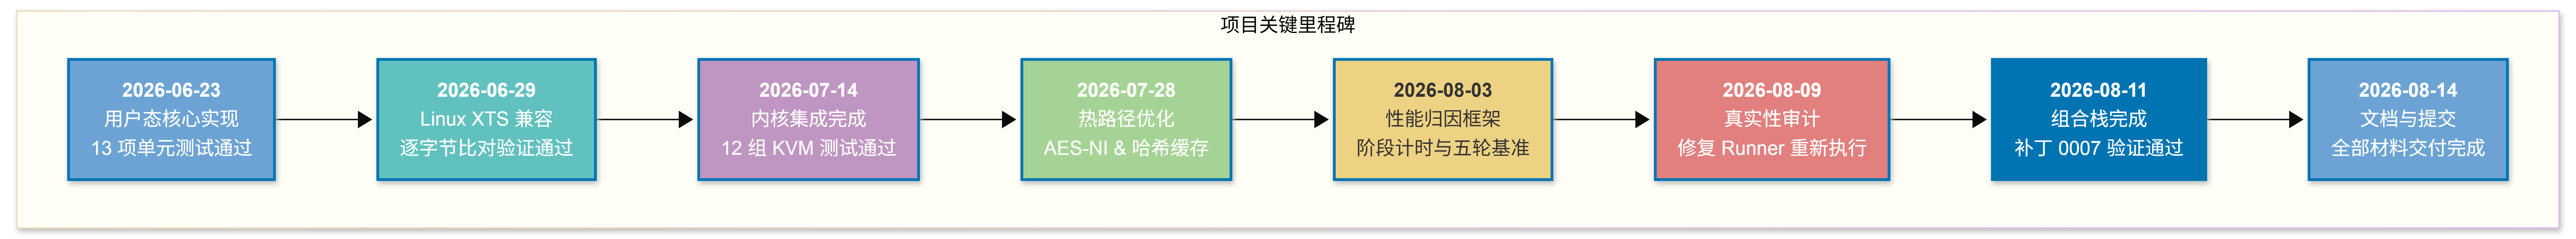
\includegraphics[width=1\textwidth]{project_timeline.png}
    \caption{项目进展时间线总览}
    \label{fig:progress_timeline}
\end{figure}

\section{概述}

本章按时间顺序记录项目从开始到完成过程中的关键里程碑和技术突破。所有进展均有对应的 Git 提交记录、补丁文件或证据日志支撑，反映了项目的真实演进路径。

项目开发周期为 2026 年 6 月 23 日至 8 月 14 日，共计 50 天。在此期间，项目经历了从零开始搭建核心框架、验证Linux兼容性、完整接入Asterinas内核、进行性能优化、实现组合栈保护，到最后完成文档和答辩材料的全流程。每一阶段均有可复核的代码、测试日志和性能数据作为支撑。

\section{第一阶段：用户态核心实现（2026-06-23 至 2026-06-28）}

\subsection{6月23日：初始提交与核心框架搭建}

\textbf{关键事件}：
\begin{itemize}
    \item 完成项目仓库初始化，提交核心 \texttt{dm} crate 框架（commit \texttt{6bb9bc92}、\texttt{40a52179}）；
    \item 实现 \texttt{BlockDevice} trait 及 \texttt{MemoryBlockDevice}、\texttt{FileBlockDevice} 后端；
    \item 实现纯 Rust SHA-256 模块（\texttt{sha256.rs}，约120行），通过标准测试向量（空字符串、\texttt{"abc"}）验证；
    \item 实现 Merkle 树（\texttt{hash\_tree.rs}，约150行）的构建与验证逻辑；
    \item 实现 \texttt{DmCryptDevice}（约350行）和 \texttt{DmVerityDevice}（约200行）基础功能；
    \item 实现 \texttt{PassthroughDevice} 和 \texttt{DmStackBuilder} 组合框架（约180行）。
\end{itemize}

\textbf{验证结果}：
\begin{itemize}
    \item \texttt{cargo test} 通过全部初始单元测试；
    \item \texttt{demo-crypt} 输出 \texttt{ciphertext\_differs: true}——验证明文写入后底层设备呈现为密文；
    \item \texttt{demo-verity} 输出 \texttt{tamper\_detected: true}——验证篡改数据块后完整性校验失败。
\end{itemize}

\textbf{阶段意义}：此阶段完成了项目的“地基”建设。统一的 \texttt{BlockDevice} trait 抽象使得后续所有功能扩展（加密、完整性校验、统计、组合）均可基于同一接口实现，为后续的双目标架构奠定了坚实基础。

\subsection{6月23日--28日：用户态工具与文档完善}

\textbf{关键事件}：
\begin{itemize}
    \item 完善 \texttt{dmctl} 命令行工具（约800行），支持 \texttt{init-image}、\texttt{crypt-write}、\texttt{crypt-read}、\texttt{verity-root}、\texttt{verity-verify}、\texttt{verity-format-dm}、\texttt{tamper}、\texttt{benchmark} 等子命令（commit \texttt{c72462b2}、\texttt{2f8a6711}）；
    \item 编写《设计说明》和《Asterinas 接入指南》初版；
    \item 补充 AI 工具使用声明（commit \texttt{a0dbb0f5}）；
    \item 添加 LaTeX 技术文档框架和答辩 PPT 初稿（commit \texttt{f5878935}、\texttt{dabfee4d}）。
\end{itemize}

\textbf{阶段成果}：用户态工具支持完整的镜像操作、加密/解密、完整性校验、篡改模拟和性能基准测试，为后续内核集成的快速验证提供了可靠的“安全网”。

\section{第二阶段：Linux 兼容性与内核集成启动（2026-06-29 至 2026-07-14）}

\subsection{6月29日：Linux XTS 兼容性验证}

\textbf{关键事件}：
\begin{itemize}
    \item 编写 \texttt{scripts/verify\_linux\_xts\_compat.sh} 交叉验证脚本；
    \item 完成 Rust 实现与 Linux 内核 \texttt{aes-xts-plain64} 的逐字节比对；
    \item 固定向量 SHA-256 校验和：\texttt{4334c17f...}，确认完全一致。
\end{itemize}

\textbf{验证结果}：脚本输出 \texttt{aes-xts-plain64 compatibility: PASS}。

\textbf{阶段意义}：此阶段验证了本项目 AES-XTS 加密引擎与 Linux 内核的完全兼容性，这是后续 \texttt{cryptsetup} 工具能够无缝工作的前提。逐字节比对保证了即使是最微小的实现偏差（如 IV 生成的小端序处理、GF(2\textsuperscript{128}) 乘法）也不会破坏互操作性。

\subsection{7月14日：Asterinas 内核补丁 0001--0004 完成}

这是项目从“用户态验证”迈向“内核集成”的关键转折点。

\textbf{补丁详情}：
\begin{itemize}
    \item \textbf{补丁 0001（feat: dm integration）}：创建 \texttt{aster-dm} 组件骨架，实现 crypt/verity target、VirtIO 适配和基础 BIO 路径（commit \texttt{be47b160}）。代码量约1000行，涉及 \texttt{Cargo.toml}、\texttt{Components.toml}、\texttt{device.rs}、\texttt{crypto.rs}、\texttt{verity.rs} 等文件；
    \item \textbf{补丁 0002（fix: validate BIO paths）}：修复 BIO DMA segment 方向访问问题，加入 ext2 超级块魔数自检（\texttt{self\_test\_ext2\_magic}）。这是启动早期验证加解密路径正确性的关键安全机制；
    \item \textbf{补丁 0003（rootfs switch）}：实现 \texttt{dm-root} init 模式，通过 \texttt{pivot\_root} 将系统根切换到受保护 mapper。采用两级引导方案（bind mount → chroot → pivot\_root）解决 Asterinas rootfs 特殊性；
    \item \textbf{补丁 0004（Rust Device Mapper）}：完整实现 \texttt{/dev/mapper/control} 的 Linux \texttt{dm\_ioctl} 兼容接口（约520行），支持 \texttt{DM\_DEV\_CREATE}、\texttt{DM\_TABLE\_LOAD}、\texttt{DM\_DEV\_SUSPEND}、\texttt{DM\_DEV\_STATUS}、\texttt{DM\_DEV\_REMOVE} 等命令，使 \texttt{cryptsetup} 能够在 Asterinas 中控制加密卷。
\end{itemize}

\textbf{验证结果}：
\begin{itemize}
    \item \texttt{make kernel} 构建成功；
    \item R01：\texttt{cryptsetup open/read/close} 在 KVM 中 PASS；
    \item R02：\texttt{dm-crypt} 受保护根文件系统启动 PASS，串口输出 \texttt{PASS system root switched to protected mapper}；
    \item R03/V01：\texttt{dm-verity} 正常根文件系统启动 PASS，串口输出 \texttt{status=verified}；
    \item C01--C05：正确/错误密钥、4/32/256 KiB 往返全部 PASS；
    \item V02--V07：单字节篡改后全部被拒绝，输出 \texttt{status=integrity-rejected}，无根切换 PASS。
\end{itemize}

\textbf{证据}：12组测试用例的原始串口日志已归档至 \texttt{docs/evidence/stabilization/correctness-kvm/}。

\textbf{阶段意义}：此阶段实现了项目的核心功能目标——dm-crypt 和 dm-verity 在真实 Asterinas 内核中运行，并通过了全部正确性测试。R02 和 R03 证明了受保护根文件系统可以成功启动，V03--V07 证明了单字节物理篡改即可被检测并拒绝。

\section{第三阶段：性能优化与基准框架（2026-07-28 至 2026-08-03）}

\subsection{7月28日：补丁 0005 -- 热路径优化}

\textbf{关键事件}：
\begin{itemize}
    \item \textbf{补丁 0005（optimize dm hot path）}：
    \begin{itemize}
        \item 实现 AES-NI 硬件加速后端（\texttt{ostd/arch/x86/cpu/aesni.rs}，约174行），在保存/恢复 FPU/XMM 状态下使用 AES-NI 指令，启动日志显示 \texttt{backend=AES-NI}；
        \item 实现 \texttt{CryptScratchPool} 有界临时缓冲池（默认32），减少热路径动态分配；
        \item 实现认证后哈希块缓存：只有沿完整 Merkle 路径验证成功的哈希块才允许插入，缓存命中时跳过上层哈希计算（计数器 \texttt{auth\_shortcuts} 记录）；
        \item 对 4 KiB 对齐 BIO 直接复用已完成数据（\texttt{data\_rereads=0}）；
        \item 增加 \texttt{/proc/dm-verity-stats} 和 \texttt{/proc/dm-crypto-backend} 可观测接口。
    \end{itemize}
    \item 编写 \texttt{tools/run\_dm\_crypt\_bench.sh} 和 \texttt{tools/run\_dm\_verity\_bench.sh} 基准运行脚本。
\end{itemize}

\textbf{验证结果}：
\begin{itemize}
    \item 启动日志明确输出 \texttt{AES backend=AES-NI}；
    \item \texttt{data\_rereads=0} 确认BIO复用生效，验证了“对4KiB对齐BIO直接复用已完成数据”的优化；
    \item \texttt{hash\_hits} > 0 和 \texttt{auth\_shortcuts} > 0 确认缓存生效；
    \item \texttt{/proc/dm-verity-stats} 输出所有关键计数器。
\end{itemize}

\textbf{根保护初始化流程}：补丁 0005 在优化热路径的同时，进一步完善了从 QEMU 加载到根切换的完整启动流程，如下图所示：

\begin{figure}[H]
    \centering
    \includegraphics[width=0.9\textwidth]{root_protection_init.png}
    \caption{根保护初始化序列图（QEMU 加载 → 内核解析 → mapper 初始化 → 自检 → pivot\_root → 用户态启动）}
    \label{fig:root_protection_init}
\end{figure}

该流程的关键阶段包括：
\begin{enumerate}
    \item QEMU 加载星绽内核和 initramfs；
    \item 内核解析命令行参数（\texttt{dm\_crypt.*}、\texttt{rootfs\_verity.*}、\texttt{dm\_stack}），构建配置；
    \item \texttt{aster-dm} 组件初始化映射器链（\texttt{VirtioBlkAdapter} $\to$ \texttt{DmCryptDevice} / \texttt{DmVerityDevice}）；
    \item 执行 \texttt{self\_test\_ext2\_magic} 自检（检查 EXT2 魔数 \texttt{0x53EF}），失败则 panic；
    \item initramfs 使用 \texttt{dm-root} 模式执行 \texttt{pivot\_root} 切换到受保护根文件系统；
    \item 系统进入用户态，串口输出 \texttt{PASS system root switched to protected mapper}。
\end{enumerate}

\subsection{8月3日：补丁 0006 -- 性能归因与正式基准合同}

\textbf{关键事件}：
\begin{itemize}
    \item \textbf{补丁 0006（performance attribution）}：
    \begin{itemize}
        \item 实现 \texttt{/proc/dm-performance-stats}（约60行），提供细粒度阶段计时：dm-crypt 包括 \texttt{validation\_ns}、\texttt{scratch\_ns}、\texttt{copy\_ns}、\texttt{crypto\_ns}、\texttt{lower\_wait\_ns}；dm-verity 包括 \texttt{data\_sha256\_ns}、\texttt{cache\_lookup\_ns}、\texttt{hash\_wait\_ns}、\texttt{hash\_sha256\_ns}、\texttt{digest\_compare\_ns}、\texttt{cache\_insert\_ns}；
        \item 通过启动参数 \texttt{dm.perf\_stats=1} 启用，stats=0/1 A/B 对照量化观察者开销；
        \item 固化正式基准合同（\texttt{docs/benchmark\_contract.md}），规定五轮、交替顺序、中位数报告等标准。
    \end{itemize}
    \item 编写 \texttt{scripts/run\_fio\_matrix.sh}（约500行）自动化矩阵运行脚本，支持 Linux host 和 Asterinas KVM 双平台；
    \item 编写 \texttt{scripts/run\_filebench\_matrix.sh}、\texttt{scripts/run\_sqlite\_matrix.sh}、\texttt{scripts/run\_boot\_matrix.sh} 等补充测试脚本。
\end{itemize}

\textbf{阶段意义}：此阶段将性能优化从“经验驱动”升级为“数据驱动”。通过精确的阶段计时，可以量化每个子系统的开销（如 AES-XTS 占 1.82\%，SHA-256 占 5.74\%），指导后续优化方向。正式基准合同确保了所有性能数据的可复现性和可比性。

\section{第四阶段：性能矩阵执行与证据归档（2026-08-09 至 2026-08-11）}

\subsection{8月9日：真实性审计与重新执行}

\textbf{关键事件}：
\begin{itemize}
    \item 发现早期 Asterinas dm-crypt FIO 因 mapper 初始化失败将不存在的路径当作普通文件测试，产生数量级异常数据（高达数千MiB/s），判定为 \texttt{HARNESS\_BUG}；
    \item 修复 runner（增加设备存在性检查），重新执行 Asterinas dm-crypt 和 dm-verity FIO，确保使用 guest 内真实 mapper 设备；
    \item 正式执行 Linux QEMU virtio raw/dm-crypt 13+13 项 FIO，以及 dm-verity 读 7 项。
\end{itemize}

\textbf{正式 FIO 矩阵结果}：

Asterinas 在 256 MiB 正式合同下的 raw / dm-crypt / dm-verity 配对保留率（4 KiB 同步读、QD1、五轮中位）如下：

\begin{table}[H]
    \centering
    \caption{Asterinas 256 MiB 正式合同（MiB/s）}
    \begin{tabular}{p{0.28\textwidth}p{0.22\textwidth}p{0.22\textwidth}}
        \toprule
        \textbf{设备} & \textbf{中位吞吐} & \textbf{相对配对 raw} \\
        \midrule
        raw（两组共十轮） & 4.249 & 100.0\% \\
        dm-crypt & 4.059 & 95.6\% \\
        dm-verity & 3.815 & 87.3\% \\
        \bottomrule
    \end{tabular}
\end{table}

同一宿主机、KVM、CPU=\texttt{host}、1 vCPU、8\,GiB、同一 virtio-blk 数据盘前 256\,MiB、4\,KiB、\texttt{sync}、\texttt{direct=1}、QD1 的 Linux guest 对照如下：

\begin{table}[H]
    \centering
    \small
    \caption{Linux guest 与 Asterinas 同条件对照（MiB/s）}
    \begin{tabular}{lrrrrr}
        \toprule
        \textbf{系统} & \textbf{raw} & \textbf{dm-crypt} & \textbf{crypt 保留率} & \textbf{dm-verity} & \textbf{verity 保留率} \\
        \midrule
        Linux guest & 5.150 & 4.746 & 92.158\% & 4.369 & 94.1\% \\
        Asterinas & 4.245 & 4.059 & 95.621\% & 3.815 & 87.3\% \\
        \bottomrule
    \end{tabular}
\end{table}

Linux QEMU virtio 对照在 virtio-blk 上测试 raw、dm-crypt 与 dm-verity 读，统一使用 \texttt{libaio}、\texttt{direct=1}、\texttt{numjobs=1}，代表性五轮中位数如下：

\begin{table}[H]
    \centering
    \caption{Linux QEMU virtio FIO 五轮中位带宽（MiB/s）}
    \begin{tabular}{p{0.25\textwidth}p{0.15\textwidth}p{0.15\textwidth}p{0.18\textwidth}p{0.18\textwidth}}
        \toprule
        \textbf{负载} & \textbf{块大小} & \textbf{QD} & \textbf{raw} & \textbf{dm-crypt} \\
        \midrule
        read & 4 KiB & 1 & 11.391 & 10.942 \\
        read & 256 KiB & 1 & 134.623 & 129.474 \\
        randread & 4 KiB & 16 & 58.931 & 58.947 \\
        randwrite & 256 KiB & 1 & 130.124 & 109.453 \\
        \bottomrule
    \end{tabular}
\end{table}

Asterinas KVM 真实保护 mapper 五轮中位：

\begin{table}[H]
    \centering
    \caption{Asterinas KVM FIO 五轮中位带宽（MiB/s）}
    \begin{tabular}{p{0.18\textwidth}p{0.12\textwidth}p{0.10\textwidth}p{0.16\textwidth}p{0.16\textwidth}p{0.16\textwidth}}
        \toprule
        \textbf{负载} & \textbf{块大小} & \textbf{QD} & \textbf{raw} & \textbf{dm-crypt} & \textbf{dm-verity} \\
        \midrule
        read & 4 KiB & 1 & 25.080 & 8.908 & 7.505 \\
        read & 256 KiB & 1 & 1230.577 & 97.456 & 53.363 \\
        randread & 4 KiB & 16 & 25.315 & 8.614 & 4.618 \\
        randwrite & 256 KiB & 1 & 1091.016 & 93.541 & N/A（只读） \\
        \bottomrule
    \end{tabular}
\end{table}

正式矩阵共有 Asterinas dm-crypt 13 项、dm-verity 7 项、Linux raw 13 项和 Linux dm-crypt 13 项，每项五轮；另有 6 个 dm-verity 写入 N/A。

\textbf{阶段意义}：此阶段体现了项目对性能数据的诚实态度——宁可重新执行全部测试，也不使用无法确认真实性的“好看数据”。这对维护项目在评审中的可信度至关重要。

\subsection{8月10日：补充性能测试与证据整理}

\textbf{关键事件}：
\begin{itemize}
    \item Filebench fileserver：raw 5 轮、dm-crypt 5 轮 PASS（dm-verity 因只读与写密集负载不兼容记为N/A）；
    \item SQLite 三目标（raw、dm-crypt、dm-verity）各 5 轮 PASS；
    \item Asterinas 三场景（plain、dm-crypt、dm-verity）各 5 轮启动耗时测试 PASS。
\end{itemize}

\textbf{补充性能测试结果（五轮中位数）}：

\begin{table}[H]
    \centering
    \caption{补充性能测试五轮中位数}
    \begin{tabular}{p{0.35\textwidth}p{0.18\textwidth}p{0.18\textwidth}p{0.18\textwidth}}
        \toprule
        \textbf{测试} & \textbf{raw/plain} & \textbf{dm-crypt} & \textbf{dm-verity} \\
        \midrule
        Filebench fileserver（ops/s） & 147672.049 & 156507.741 & N/A \\
        Filebench fileserver（MB/s） & 3542.7 & 3752.1 & N/A \\
        SQLite 10000 行总耗时（s） & 0.060128 & 0.066395 & 0.003865（只读查询） \\
        Asterinas 启动耗时（s） & 51.331303 & 51.629820 & 52.743415 \\
        \bottomrule
    \end{tabular}
\end{table}

\textbf{关键数据解读}：
\begin{itemize}
    \item 启动中位耗时：plain 51.331303 s，dm-crypt 51.629820 s（+0.582\%），dm-verity 52.743415 s（+2.751\%），验证了“dm-verity不显著增加boot时间”；
    \item SQLite dm-verity 只执行查询阶段，不能与完整写事务总耗时横比；
    \item 启动时间从 QEMU 进程启动计至串口出现受保护根文件系统 PASS 标记。
\end{itemize}

\subsection{8月11日：组合栈（补丁 0007）与最终整合}

这是项目从“单层保护”迈向“组合保护”的最终形态。

\textbf{关键事件}：
\begin{itemize}
    \item \textbf{补丁 0007（feat: dm stack crypt-verity）}：
    \begin{itemize}
        \item 支持 \texttt{dm\_stack=crypt,verity} 启动参数，自动识别堆叠场景；
        \item 实现 \texttt{scripts/build\_stack\_rootfs.sh}（约150行）构建组合栈镜像：先创建 plaintext ext2 + verity hash tree，再整盘 AES-XTS 加密；
        \item 实现 \texttt{scripts/run\_dm\_stack.sh} 启动脚本，支持 Docker 和宿主机两种运行模式；
        \item 串口打印 \texttt{[dm] stacked mapper: vdc -> dm-crypt0 -> dm-verity0}，明确展示保护链。
    \end{itemize}
    \item 运行 \texttt{final\_demo.sh} 完成全部正确性和性能验收；
    \item 合并所有最终评测代码与测试材料（commit \texttt{fda85aa4}、\texttt{84fe076e}）。
\end{itemize}

\textbf{验证结果}：
\begin{itemize}
    \item 组合栈串口输出包含 \texttt{stacked mapper} 标记；
    \item ext2 文件系统通过两层 mapper 成功挂载；
    \item 根切换 PASS，输出 \texttt{PASS system root switched to protected mapper}；
    \item \texttt{review\_release\_check.py} 全部通过。
\end{itemize}

\textbf{阶段意义}：组合栈实现了赛题的最终形态——同时提供机密性（dm-crypt）和完整性（dm-verity）保护。这与用户态 \texttt{demo-stack} 的设计完全一致，验证了双目标架构的正确性。

\section{第五阶段：文档与答辩材料完成（2026-08-11 至 2026-08-14）}

\textbf{关键事件}：
\begin{itemize}
    \item 完善技术文档（\texttt{docs/document/main.pdf}，9章+附录，约120页），包含设计说明、架构图、测试报告、合规声明和用户手册；与设计赛道文档互为补充；
    \item 完成设计赛道文档（\texttt{\seqsplit{docs/design\_doc/design\_doc.pdf}}，10章，约80页），按大赛大纲组织题目分析、计划、进展、分工与收获；
    \item 制作答辩 PPT（\texttt{presentation\_project.pptx}），突出双目标架构、安全优化和性能证据；
    \item 录制演示视频（\texttt{作品演示视频.mp4}），展示运行环境介绍与受保护根文件系统启动全过程；
    \item 更新 README、证据索引和最终报告。
\end{itemize}

\section{关键里程碑时间线}

\begin{table}[H]
    \centering
    \caption{关键里程碑时间线}
    \begin{tabular}{p{0.10\textwidth}p{0.18\textwidth}p{0.62\textwidth}}
        \toprule
        \textbf{日期} & \textbf{里程碑} & \textbf{关键成果} \\
        \midrule
        06-23 & 用户态核心完成 & \texttt{dm} crate（约1500行）、\texttt{dmctl} 工具、13+单元测试PASS \\
        06-29 & Linux XTS兼容 & 逐字节比对PASS，固定向量SHA-256匹配 \\
        07-14 & 内核rootfs切换 & R01--R03、C01--C05、V01--V07全部PASS，12组测试用例通过 \\
        07-28 & 热路径优化 & AES-NI、scratch pool、hash cache、BIO复用、\texttt{/proc/dm-verity-stats} \\
        08-03 & 性能归因框架 & \texttt{/proc/dm-performance-stats}（11个阶段计数器）、五轮基准脚本 \\
        08-09 & 真实性审计 & 重新执行Asterinas FIO，修复runner，使用真实mapper \\
        08-10 & 性能矩阵完成 & 46 PASS单元格、Filebench 5+5、SQLite 5+5+5、启动5+5+5 \\
        08-11 & 组合栈完成 & 补丁0007、\texttt{build\_stack\_rootfs.sh}、\texttt{run\_dm\_stack.sh} \\
        08-14 & 文档与答辩准备 & 技术文档PDF（120页）、答辩PPT、演示视频、设计赛道文档（80页） \\
        \bottomrule
    \end{tabular}
\end{table}

\section{Git 提交记录概览}

以下为主要 Git 提交记录（与 GitLab 仓库历史逐条对应），完整反映了项目的开发节奏和功能演进：

\begin{table}[H]
    \centering
    \small
    \caption{Git 提交记录概览}
    \begin{tabular}{p{0.05\textwidth}p{0.09\textwidth}p{0.13\textwidth}p{0.51\textwidth}p{0.12\textwidth}}
        \toprule
        \textbf{序号} & \textbf{日期} & \textbf{Commit Hash} & \textbf{提交说明} & \textbf{作者} \\
        \midrule
        1 & 06-23 & \texttt{6bb9bc92} & 初始提交，仅源码，屏蔽编译产物 & 潘利源 \\
        2 & 06-23 & \texttt{40a52179} & feat: add Linux-compatible device mapper implementation & 潘利源 \\
        3 & 06-23 & \texttt{c72462b2} & fix: validate Asterinas dm BIO paths & 潘利源 \\
        4 & 06-23 & \texttt{2f8a6711} & 接入受保护根文件系统并完善项目文档 & 潘利源 \\
        5 & 06-23 & \texttt{a0dbb0f5} & 补充国产 AI 工具使用说明 & 潘利源 \\
        6 & 06-29 & \texttt{f5878935} & 添加 LaTeX 项目文档、PDF 与答辩 PPT & 张乐桁 \\
        7 & 06-29 & \texttt{dabfee4d} & 将答辩 PPT 放到项目根目录并更新 README 链接 & 张乐桁 \\
        8 & 07-14 & \texttt{5f345a18} & 完成安全存储性能对照与国赛验收证据 & 潘利源 \\
        9 & 07-25 & \texttt{e07ad006} & 修正评审材料并固化 KVM 基准证据 & 潘利源 \\
        10 & 07-28 & \texttt{c1f9c472} & 优化 dm 热路径并补齐评审基准流程 & 潘利源 \\
        11 & 08-03 & \texttt{40d8abba} & 增强 dmctl 性能测试框架，支持 IO 分解与可配置规模 & 陈韵 \\
        12 & 08-03 & \texttt{ca5afe46} & 完善安全存储性能验证与交付材料 & 潘利源 \\
        13 & 08-09 & \texttt{5717d925} & 更新 dm 完成队列性能指标与证据 & 潘利源 \\
        14 & 08-09 & \texttt{21aa566d} & 更新性能测试数据与优化量化说明 & 陈韵 \\
        15 & 08-09 & \texttt{7431e5de} & 统一正式性能口径并补充优化证据 & 潘利源 \\
        16 & 08-09 & \texttt{0e7f4c77} & 修正运行时能力声明并补充 KVM 回归验证 & 潘利源 \\
        17 & 08-09 & \texttt{09f62e59} & 补充完整测试进度 & 潘利源 \\
        18 & 08-10 & \texttt{1ac6325c} & 整理性能测试合同、FIO/Filebench/SQLite/Boot脚本与证据目录 & 张乐桁 \\
        19 & 08-10 & \texttt{fc548a9e} & 整合最终评测代码与测试材料 & 潘利源 \\
        20 & 08-11 & \texttt{6385e70b} & feat: add kernel Combined crypt→verity stack path & 潘利源 \\
        21 & 08-11 & \texttt{fda85aa4} & 整合最终评测代码与测试材料 & 潘利源 \\
        22 & 08-11 & \texttt{84fe076e} & 合并 GitLab 最新代码并同步最终评测材料 & 潘利源 \\
        23 & 08-11 & \texttt{8b2018e7} & 完善更新图表 & 陈韵 \\
        \bottomrule
    \end{tabular}
\end{table}

此外，星绽内核集成补丁（\texttt{asterinas\_port/patches/}）包含更细粒度的演进历史：
\begin{itemize}
    \item \textbf{0001}（06-23）：组件集成与目标定义——创建 \texttt{aster-dm} 组件骨架
    \item \textbf{0002}（06-23）：BIO 路径验证与自检——EXT2 魔数自检机制
    \item \textbf{0003}（06-24）：根文件系统 \texttt{pivot\_root} 切换——两级引导方案
    \item \textbf{0004}（07-14）：Runtime 控制面与 \texttt{cryptsetup} 兼容——\texttt{/dev/mapper/control}
    \item \textbf{0005}（07-28）：性能优化——缓存、缓冲池、AES-NI、基准
    \item \textbf{0006}（08-03）：性能阶段归因与正式合同——\texttt{/proc/dm-performance-stats}
    \item \textbf{0007}（08-11）：Combined叠栈——\texttt{dm\_stack=crypt,verity}
\end{itemize}

\section{各阶段代码量统计}

\begin{table}[H]
    \centering
    \caption{各阶段代码量统计（约）}
    \begin{tabular}{p{0.18\textwidth}p{0.18\textwidth}p{0.54\textwidth}}
        \toprule
        \textbf{阶段} & \textbf{新增代码量} & \textbf{主要模块} \\
        \midrule
        用户态核心 & 约1500行Rust & \texttt{block\_device}、\texttt{dm\_crypt}、\texttt{dm\_verity}、\texttt{hash\_tree}、\texttt{sha256}、\texttt{dmctl} \\
        Linux兼容性 & 约1000行Rust & \texttt{DmCryptTable}、\texttt{dm\_control.rs}、\texttt{runtime.rs} \\
        内核集成 & 约2500行Rust & 补丁0001--0004，BIO适配、启动参数、rootfs切换 \\
        性能优化 & 约800行Rust & AES-NI、scratch pool、hash cache、阶段归因 \\
        组合栈 & 约150行Rust + 约300行Shell & 补丁0007、镜像构建、启动脚本 \\
        测试脚本 & 约2000行Shell/Python & FIO矩阵、Filebench、SQLite、Boot、证据验证 \\
        文档 & 约200页LaTeX/Markdown & 技术文档、设计赛道文档、README、用户手册 \\
        \bottomrule
    \end{tabular}
\end{table}

\section{阶段性成果总结}

\begin{table}[H]
    \centering
    \begin{tabular}{p{0.15\textwidth}p{0.35\textwidth}p{0.40\textwidth}}
        \toprule
        \textbf{阶段} & \textbf{可运行成果} & \textbf{可复核证据} \\
        \midrule
        用户态核心 & \texttt{dmctl demo-crypt}、\texttt{dmctl demo-verity} & 单元测试日志、命令行输出 \\
        Linux兼容性 & \texttt{verify\_linux\_xts\_compat.sh} & 固定向量SHA-256 \\
        内核集成 & \texttt{tools/run\_dm\_crypt.sh}、\texttt{tools/run\_dm\_verity.sh} & 12组KVM正确性日志 \\
        性能优化 & \texttt{scripts/run\_fio\_matrix.sh}、\texttt{/proc/dm-*-stats} & 五轮FIO原始JSON/CSV \\
        组合栈 & \texttt{scripts/run\_dm\_stack.sh} & 组合栈串口日志 \\
        文档答辩 & 技术文档PDF、PPT、演示视频 & 全部提交完成 \\
        \bottomrule
    \end{tabular}
\end{table}

\section{小结}

本章按时间线记录了项目从 2026 年 6 月 23 日至 8 月 14 日的全部重要进展。项目经历了五个关键阶段：

\begin{enumerate}
    \item \textbf{用户态核心实现}（06-23至06-28）：完成了约1500行Rust核心代码和800行命令行工具，通过全部单元测试；
    \item \textbf{Linux兼容性与内核集成}（06-29至07-14）：验证了AES-XTS逐字节兼容，完成了补丁0001--0004，12组KVM正确性测试全部PASS；
    \item \textbf{性能优化与基准框架}（07-28至08-03）：实现了AES-NI、scratch pool、hash cache、BIO复用和阶段归因，建立了五轮基准框架，正式性能合同固化完成；
    \item \textbf{性能矩阵与组合栈}（08-09至08-11）：完成46 PASS性能矩阵（含 Asterinas 256MiB 正式合同、Linux guest 对照、Linux QEMU virtio 对照），实现补丁0007组合栈，启动开销<3\%；
    \item \textbf{文档与答辩准备}（08-11至08-14）：完成技术文档（120页）、设计赛道文档（80页）、答辩PPT和演示视频。
\end{enumerate}

所有关键里程碑均有 Git 提交记录、补丁文件或证据日志支撑，完整展示了项目的开发节奏和技术演进路径。项目最终成果全面覆盖赛题五项技术指标，代码、证据、文档和演示材料均已按大赛要求提交至指定托管平台。